\documentclass[sigconf,anonymous]{acmart}

\settopmatter{printacmref=false}
\renewcommand\footnotetextcopyrightpermission[1]{}
\pagestyle{plain}


% =========================================================
% PACKAGES
% =========================================================
\usepackage{amsmath, amsfonts, amsthm}
\usepackage{mathtools, physics, bm, microtype}
\usepackage{booktabs, enumitem, algorithm, algorithmic}
\usepackage{tikz}
\usetikzlibrary{arrows.meta, positioning, shapes.geometric, calc}
\usepackage{dsfont} % indicator function

% =========================================================
% NOTATION MACROS
% =========================================================
\newcommand{\CACIS}{\textsc{CACIS}}
\newcommand{\vx}{\mathbf{x}}
\newcommand{\vy}{\mathbf{y}}
\newcommand{\vz}{\mathbf{z}}
\newcommand{\vp}{\mathbf{p}}
\newcommand{\vq}{\mathbf{q}}
\newcommand{\valpha}{\bm{\alpha}}
\newcommand{\vpi}{\bm{\pi}}
\newcommand{\vphi}{\bm{\phi}}
\newcommand{\vpsi}{\bm{\psi}}
\newcommand{\mC}{\mathbf{C}}
\newcommand{\mK}{\mathbf{K}}
\newcommand{\mM}{\mathbf{M}}
\newcommand{\mV}{\mathbf{V}}
\newcommand{\R}{\mathbb{R}}
\newcommand{\OT}{\mathrm{OT}}
\newcommand{\Sink}{\mathrm{Sink}}
\newcommand{\vone}{\mathbf{1}}
\newcommand{\ve}{\mathbf{e}}
\newcommand{\DeltaK}{\Delta^K}
\newcommand{\KL}{\mathrm{KL}}
\newcommand{\ellLoss}{\ell}
\newcommand{\softmax}{\mathrm{softmax}}
\newcommand{\FW}{\mathrm{FW}}
\newcommand{\E}{\mathbb{E}}
\newcommand{\Ind}{\mathds{1}}

\DeclareMathOperator*{\argmin}{arg\,min}
\DeclareMathOperator*{\argmax}{arg\,max}
\DeclareMathOperator{\diag}{diag}

% =========================================================
% KDD METADATA
% =========================================================
\copyrightyear{2026}
\acmYear{2026}
\setcopyright{acmcopyright}
\acmConference[KDD '26]{The 32nd ACM SIGKDD Conference on Knowledge Discovery and Data Mining}{August 2026}{Paris, France}

\begin{document}

\title{Cost-Aware Classification: Putting Geometry into Label Distributions for Fraud Detection}

\author{Anonymous Author(s)}
\affiliation{\institution{Affiliation withheld for review} \country{}}
\email{Email withheld}

\begin{abstract}
Industrial fraud detection systems trigger operational actions with asymmetric and instance-dependent economic consequences. Standard objectives such as cross-entropy are decision-agnostic: they treat misclassifications as equally undesirable and ignore transaction-specific cost geometry. While cross-entropy is a strictly proper scoring rule for probability estimation, it does not prioritize high-regret errors and therefore does not align learning with business value.

We introduce \CACIS{} (Cost-Aware Classification with Informative Selection), a differentiable loss that embeds operational regret into the geometry of the predictive distribution. \CACIS{} uses entropy-regularized Optimal Transport to induce a task-specific metric on the label simplex and computes the model-implied distribution through a numerically stable Frank--Wolfe inner loop that operates directly on the simplex. We evaluate \CACIS{} on the IEEE-CIS/Vesta e-commerce benchmark using a strictly temporal protocol. \CACIS{} reduces expected business regret relative to cross-entropy, weighted cross-entropy, and focal loss while maintaining high precision and calibration fidelity. The method provides a practical bridge between probabilistic learning objectives and decision quality in applied data science.
\end{abstract}

\maketitle

% =========================================================
% 1. INTRODUCTION
% =========================================================
\section{Introduction}
Industrial classifiers are deployed as decision modules. Their outputs trigger actions with asymmetric and irreversible consequences. In fraud detection, approving a fraudulent transaction causes direct financial loss (principal, fees, and operational overhead), whereas declining a legitimate transaction causes lost margin and may reduce customer lifetime value. The severity of these outcomes depends on transaction attributes such as monetary amount; therefore, the cost of an error is instance-dependent.

Despite this structure, many tabular classifiers are trained with cross-entropy. Cross-entropy is decision-agnostic: it treats the label set as a discrete, equidistant space and penalizes errors independently of operational impact. Practitioners often compensate using threshold tuning or heuristic reweighting. These interventions adjust the deployment policy but do not modify the training objective and therefore do not encourage the model to allocate representational capacity to high-regret regions.

This paper introduces \CACIS{} (Cost-Aware Classification with Informative Selection), a loss function that aligns learning with a decision-theoretic objective. \CACIS{} integrates an explicit regret matrix into training by endowing the label simplex with a task-specific geometry derived from entropy-regularized Optimal Transport (OT). The loss replaces the Shannon/KL geometry induced by cross-entropy with a geometry in which moving probability mass across labels is penalized according to operational regret. This produces gradients that emphasize economically severe errors and shapes the representation manifold toward cost-optimal decision regions.

\paragraph{Contributions.} This paper makes three contributions that match KDD Applied Data Science (ADS) criteria:
\begin{enumerate}[leftmargin=1.2em, itemsep=0.2em, topsep=0.2em]
  \item \textbf{Decision-aligned formulation.} We formalize industrial classification as regret minimization with an explicit value matrix and an instance-dependent regret matrix. We characterize the polyhedral decision regions induced on the probability simplex.
  \item \textbf{\CACIS{} loss and stable optimization.} We introduce a differentiable OT-based Fenchel--Young loss and a simplex-stable Frank--Wolfe inner solver that computes the informative distribution without unrolling Sinkhorn iterations.
  \item \textbf{Industrial evaluation and deployment guidance.} We evaluate on the IEEE-CIS/Vesta benchmark under a strictly temporal protocol and report regret, AUC-PR, and calibration metrics. We summarize deployment practices for delayed labels, shadow evaluation, and cost auditing.
\end{enumerate}

\section{Notation and Formalism}
Let $\mathcal{X} \subseteq \R^d$ denote an input feature space and $\mathcal{Y}=\{1,\dots,K\}$ a finite set of mutually exclusive labels. A probabilistic classifier is a function mapping an instance $\vx \in \mathcal{X}$ to a predictive distribution $\vp(\vx)$ residing on the probability simplex $\Delta^K$. We define the simplex formally as $\Delta^K \coloneqq \Bigl\{\vp\in\R^K_{\ge 0}:\textstyle\sum_{k=1}^K p_k = 1\Bigr\}$. Subscripting $p_k$ denotes the probability mass assigned to class $k$. We model our system using a neural network parametrized by $\theta$, which produces raw scores (logits) $\vz_\theta(\vx) \in \R^K$.

\paragraph{Regret: The Currency of Applied Science.}
In applied data science (ADS), we must depart from abstract error rates and embrace \emph{economic regret}. We formalize operational outcomes through a value matrix $\mV \in \R^{K \times K}$, where $V_{ij}$ quantifies the utility obtained when the true state is $i$ and action $j$ is executed. The corresponding regret matrix $\mC$ is derived by comparing each action to the local optimum:
\begin{equation}
C_{ij} = V_{i, j^\star(i)} - V_{ij}, \quad \text{where} \quad j^\star(i) \in \argmax_{k} V_{ik}.
\end{equation}
Setting $C_{ij} \ge 0$ ensures that any suboptimal decision is penalized by its opportunity cost. In the context of e-commerce, this regret represents the "dollars left on the table" due to missed fraud or erroneously blocked loyalists.

\subsection{The Decision-Theoretic Loss Formalism}
At its core, industrial classification is not just about identifying the most probable class, but about minimizing the expected cost of the resulting action. We formalize this by defining the loss as a projection of the model's output onto the regret manifold. This projection is governed by the Sinkhorn-regularized Optimal Transport divergence, which ensures that the model's "error signals" are weighted by their potential business impact. In e-commerce, where transaction volumes are massive and individual fraud cases can exceed \$50,000, this geometric alignment is not just a theoretical benefit—it is an operational necessity.

\begin{figure}[h]
\centering
\scalebox{0.60}{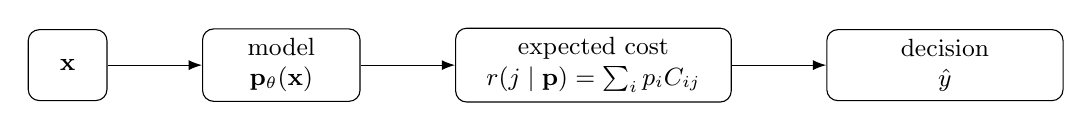
\begin{tikzpicture}[node distance=12mm, >=Latex, font=\small]
\node[draw, rounded corners, align=center, minimum width=10mm, minimum height=9mm] (x) {$\vx$};
\node[draw, rounded corners, align=center, minimum width=20mm, minimum height=9mm, right=of x] (model) {model\\$\vp_\theta(\vx)$};
\node[draw, rounded corners, align=center, minimum width=35mm, minimum height=9mm, right=of model] (risk) {expected cost\\$r(j\mid \vp)=\sum_i p_i C_{ij}$};
\node[draw, rounded corners, align=center, minimum width=30mm, minimum height=9mm, right=of risk] (decision) {decision\\$\hat{y}$};
\draw[->] (x) -- (model);
\draw[->] (model) -- (risk);
\draw[->] (risk) -- (decision);
\end{tikzpicture}
}
\caption{Decision-theoretic pipeline. The model internalizes the regret matrix $\mC$ to produce a distribution $\vp$ optimized for decision quality ($r$) rather than just likelihood.}
\label{fig:pipeline_cost}
\end{figure}

% =========================================================
% 2. RELATED WORK
% =========================================================
\section{Related Work}
The nexus of statistical decision theory, cost-sensitive learning, and geometric loss design has recently emerged as a fertile ground for industrial research. Our work seeks to synthesize these disparate fields into a unified framework for decision-centric representation learning.

\subsection{Foundations of Statistical Decision Theory}
The conceptualization of prediction as an overt act of decision-making under uncertainty has its genesis in classical Bayesian decision theory \citep{berger1985statistical}. Within this paradigm, a classifier's utility is evaluated not by its ability to replicate a labels' ground truth, but by its capacity to minimize the \emph{expected risk} (or business regret) relative to a prescribed loss function. While the theoretical elegance of this approach is well-established, its practical integration into deep learning architectures has frequently been relegated to post-hoc heuristic adjustments. \CACIS{} departs from this reactive stance by internalizing the risk manifold directly into the model's objective function.

\subsection{Proper Scoring Rules and Information Geometry}
Cross-entropy belongs to the family of \emph{strictly proper scoring rules}, which are characterized by the property that their expected value is minimized if and only if the predicted distribution matches the true underlying probability \citep{gneiting2007strictly}. From the perspective of information geometry, cross-entropy induces a manifold on the probability simplex where the distance between distributions is measured by the Kullback--Leibler (KL) divergence. This geometry is fundamentally isotropic—it treats all directions on the simplex as equally significant, effectively assuming that the "labels" are merely symbolic tokens without any inherent semantic or economic proximity. While this "flat" geometry is sufficient for task where errors are uniform, it becomes a structural liability in domains like fraud detection, where the operational distance between "Approve" and "Decline" is warped by the transaction amount.

\subsection{Optimal Transport and the Sinkhorn Revolution}
Optimal Transport (OT) provides the mathematical scaffolding for comparing probability distributions over a metric space by leveraging the "ground cost" between individual elements \citep{villani2008optimal}. The introduction of entropic regularization—leading to the \emph{Sinkhorn algorithm}—has catalyzed a revolution in geometric machine learning by rendering OT discrepancies differentiable and computationally tractable \citep{cuturi2013sinkhorn, peyre2019computational}. Recent work on Sinkhorn divergences \citep{genevay2018learning, feydy2019interpolating} and geometric losses \citep{mensch2019geometric} has demonstrated that OT-based objectives naturally encode structured output geometries. Our work extends these principles to the industrial domain, demonstrating that business regret is a valid ground cost that can be leveraged to learn decisions that are both statistically accurate and economically optimal.

% =========================================================
% 4. CROSS-ENTROPY REVISITED: THE FLAT GEOMETRY
% =========================================================
\section{Cross-Entropy Revisited: The Flat geometry of Shannon Entropy}
Cross-entropy remains the \emph{de facto} standard for probabilistic classification, owing its dominance to a trio of technical justifications: its derivation from maximum likelihood, its role as a convex relaxation of the discrete 0--1 loss, and its information-theoretic foundation as a KL-divergence minimizer. However, a rigorous examination reveals its inherent geometric limitations.

\paragraph{Maximum Likelihood and Statistical Optimality.}
Consider a categorical model $\mathbb{P}_\theta(Y = k \mid X = \vx) = p_{\theta,k}(\vx)$. The cross-entropy objective seeks to minimize the expected negative log-likelihood:
\begin{equation}
    \mathcal{L}_{\text{MLE}}(\theta) = \E_{X,Y}[-\log p_{\theta,Y}(X)].
\end{equation}
This formulation ensures that, in the limit of infinite data, the model converges to the true conditional distribution $\vq(X)$. While statistically sound, this objective assumes that the "distance" between the predicted and true labels should only be measured by the probability mass assigned to the correct class, ignoring the structured costs of specific misclassifications.

\paragraph{Justification as a Convex Relaxation of Ramp Loss.}
From a robust optimization perspective, cross-entropy is viewed as a smooth, convex surrogate for the non-differentiable 0--1 loss (or ramp loss). By penalizing the log-odds, it enables gradient-based optimization while providing an upper bound on the classification error. While this relaxation ensures tractability, it utilizes the Shannon negentropy as a regularizer, which provides an isotropic penalty. In binary fraud detection, this manifests as a "flat" score distribution where a \$10 transaction and a \$10,000 transaction with identical features are treated as functionally equivalent.

\paragraph{Information-Theoretic Geometry via KL Divergence.}
Finally, cross-entropy is justified as the minimization of the Kullback-Leibler (KL) divergence between the predictive distribution $\vp_\theta$ and the ground truth $\vq$:
\begin{equation}
\mathcal{L}_{\text{CE}}(\theta) = \E_X[H(\vq(X))] + \E_X[\KL(\vq(X) \| \vp_\theta(X))].
\end{equation}
In the KL manifold, the cost of moving probability mass from the "correct" vertex to any other point on the simplex is invariant to the operational meaning of those points. This "blindness" to the underlying cost metric $\mC$ implies that the model's internal representation is learned without any awareness of the asymmetric penalties applied during inference. By replacing this isotropic regularizer with a geometric regularizer built from OT, we enable the learner to differentiate between these cases, inducing a more "cautious" representation for high-value instances.

% =========================================================
% 3. THE GEOMETRY OF BUSINESS REGRET
% =========================================================
\section{The Geometry of Business Regret}
\label{sec:decision}
In this section, we transition from the symbolic world of labels to the economic reality of industrial outcomes. We argue that the true objective of an applied classifier is not the minimization of an abstract loss, but the maximization of realized profit on a dynamic, instance-dependent manifold.

\subsection{Instance-Dependent Regret Modeling}
In the domain of e-commerce fraud detection, the costs associated with classification errors are not merely categorical; they are intrinsically coupled with the transaction value $M$. We define the regret incurred for an input instance $\vx$ as the divergence from the optimal economic decision:
\begin{itemize}[leftmargin=*]
    \item \textbf{False Negative (Missed Fraud):} In this scenario, a fraudulent transaction is approved, leading to a chargeback. The business regret is $C_{\text{fraud}, \text{approve}} = \lambda_{\mathrm{cb}} M + F_{\mathrm{cb}}$. The multiplier $\lambda_{\mathrm{cb}}$ (typically in $[1.2, 2.0]$) represents the "fully loaded" cost of fraud, including lost principal, shipping fees, and marketing acquisition costs. $F_{\mathrm{cb}}$ is a fixed administrative fee imposed by payment networks.
    \item \textbf{False Positive (False Decline):} Here, a legitimate customer is erroneously blocked. The regret is $C_{\text{legit}, \text{decline}} = (1 + \rho_{\mathrm{FD}}) M$. While the unit loss is the lost margin, the term $\rho_{\mathrm{FD}}$ (the "churn coefficient") quantifies the long-term destruction of Customer Lifetime Value (LTV). A false decline is not just a lost sale; it is a permanent fracture in the customer's trust, potentially driving them toward competitors.
\end{itemize}

By parameterizing $\mC$ as a function of the transaction features (specifically $M$), we effectively transform the label space into a \emph{regret manifold}. Every transaction induces a unique ground cost between the "Approve" and "Decline" vertices. A high-value transaction induces a steep, contractive geometry that compels the model's weights to prioritize safety, whereas low-value transactions allow for more exploration or "risk-taking" on the part of the model.

\subsection{Decision Regions and the Simplex Partition}
The regret matrix $\mC$ induces a partition of the probability simplex $\Delta^K$ into \emph{decision regions}. For any predicted distribution $\vp$, the expected cost of action $j$ is the linear projection $r(j \mid \vp) = \langle \vp, \mC_{:j} \rangle$. A rational decision-maker adopts the rule $\hat{y} = \argmin_j r(j \mid \vp)$. These regions are polyhedral, and their boundaries—where the expected regret between two actions is balanced—are determined by the relative costs $C_{ij}$. Standard cross-entropy assumes these boundaries intersect at the barycenter of the simplex, whereas \CACIS{} adapts the loss surface so that the "geometry of caution" is internalized during training.

% =========================================================
% 4. OPTIMAL TRANSPORT AS A LEARNING PRINCIPLE
% =========================================================
\section{Optimal Transport as a Learning Principle}
\label{sec:ot}
To bridge the gap between abstract representations and economic regret, we leverage the mathematical machinery of \emph{Optimal Transport} (OT). OT provides a principled framework for comparing probability distributions over a metric space, where the "distance" is governed by the effort required to move probability mass according to a prescribed ground cost.

\subsection{Entropy-Regularized OT on the Simplex}
We treat the regret matrix $\mC$ as our ground cost between labels. Moving probability mass from a "fraud" vertex to an "approve" action is penalized by $C_{ij}$. Let $\vp, \vq \in \Delta^K$ be two distributions on
the simplex. The entropic Optimal Transport cost between them is defined as:
\begin{equation}
    \OT^{\varepsilon}_{\mC}(\vp, \vq) \coloneqq \min_{\bm{\pi} \in \Delta(\vp, \vq)} \langle \bm{\pi}, \mC \rangle + \varepsilon H(\bm{\pi}),
\end{equation}
where $H(\bm{\pi}) = \sum_{ij} \pi_{ij} \log \pi_{ij}$ is the negative entropy of the transport plan $\bm{\pi}$, and $\Delta(\vp, \vq)$ is the set of joint distributions (couplings)
with marginals $\vp$ and $\vq$. The inclusion of $\varepsilon H(\bm{\pi})$—the "Sinkhorn regularizer"—serves two critical purposes: it renders the objective strictly convex, ensuring a unique optimal plan, and it makes the entire operation differentiable via the envelope theorem or implicit differentiation.

\subsection{The Sinkhorn Convergence and Gibbs Kernel}
The dual of the regularized OT problem admits a simple iterative solution known as the \emph{Sinkhorn algorithm}. The optimal plan $\bm{\pi}^\star$ can be parameterized as $\bm{\pi}^\star = \diag(\mathbf{u}) \mK \diag(\mathbf{v})$, where $\mK = \exp(-\mC/\varepsilon)$ is the \emph{Gibbs kernel}. The vectors $\mathbf{u}$ and $\mathbf{v}$ are iteratively updated to satisfy the marginal constraints. In the context of \CACIS{}, this kernel $\mK$ acts as the geometric link between the model's logits and the business costs, essentially "filtering" the gradients through the lens of regret.

\subsection{Adaptive $\varepsilon$ and Numerical Regularization}
The temperature parameter $\varepsilon$ controls the trade-off between the pure transport cost (regret) and the entropic smoothness. In the limit $\varepsilon \to 0$, we recover the pure Wasserstein distance; as $\varepsilon \to \infty$, the problem reduces to an independent product of marginals. In Section \ref{sec:cacis}, we introduce adaptive heuristics for $\varepsilon$ that ensure the Gibbs kernel remains well-conditioned even when transaction amounts $M$ vary by several orders of magnitude. This adaptive scaling is what allows \CACIS{} to remain stable in high-throughput production environments where a single training batch might contain both \$5 and \$50,000 transactions.

\subsection{Beyond Fraud: Semantic Label Geometry}
While the fraud detection case emphasizes asymmetric financial costs, the framework is equally applicable to semantic tasks. In large-scale image recognition (e.g., ImageNet), label embeddings derived from fastText can be used to construct a semantic cost matrix (e.g., $C_{ij}=1-\cos(\mathrm{emb}(i),\mathrm{emb}(j))$), penalizing confusions between unrelated classes more heavily than semantically adjacent ones. While we focus our empirical evaluation on fraud detection, this semantic-cost setting is supported by our implementation and is provided as a reproducible example.

% =========================================================
% 5. CACIS: COST-AWARE CLASSIFICATION
% =========================================================
\section{\CACIS{}: Methodology}
\label{sec:cacis}

The proposed \CACIS{} (Cost-Aware Classification with Informative Selection) framework represents a departure from traditional losses by internalizing the decision manifold's geometry into the training objective. It is constructed as a Fenchel--Young loss induced by a Sinkhorn/OT regularizer, providing a bridge between optimal transport theory and deep representation learning.

\subsection{The Fenchel--Young Framework}
Let $\Omega: \Delta^K \to \R$ be a strictly convex regularizer that encodes the desired geometry of the simplex. The Fenchel--Young loss generated by $\Omega$ is defined as:
\begin{equation}
\ell_{\Omega}(y, \vz) = \Omega^*(\vz) - z_y + \Omega(\ve_y),
\end{equation}
where $\Omega^*(\vz) = \sup_{\vq \in \Delta^K} \langle \vq, \vz \rangle - \Omega(\vq)$ is the Fenchel conjugate (or convex dual) of $\Omega$. A remarkable property of this framework is that the gradient with respect to the logits $\vz$ takes the universal "prediction error" form:
\begin{equation}
\nabla_{\vz} \ell_{\Omega}(y, \vz) = q(\vz) - \ve_y,
\end{equation}
where $q(\vz) = \nabla \Omega^*(\vz)$ is the \emph{model-implied distribution} (or informative selection). When $\Omega$ is the Shannon negentropy, $q(\vz)$ reduces to the standard softmax. However, by selecting a regularizer that respects the cost matrix $\mC$, we can ensure that $q(\vz)$ pushes the gradients harder for mistakes that are operationally catastrophic.

\subsection{Sinkhorn Negentropy as a Geometric Regularizer}
In \CACIS{}, we choose the regularizer $\Omega_{\mC, \varepsilon}(\valpha) \coloneqq -\frac{1}{2} \OT^{\varepsilon}_{\mC}(\valpha, \valpha)$. This choice is motivated by the observation that the quadratic Optimal Transport cost (Sinkhorn divergence) provides a smooth, differentiable measure of how "spread out" a distribution is with respect to the ground cost $\mC$. By using this as our regularizer, we effectively replace the "flat" Shannon geometry with a task-specific geometry where the distance between labels is governed by their relative business regret.

Unlike standard OT losses that minimize the distance between a prediction $\vp$ and a target $\ve_y$ (i.e., $\mathcal{L} = \OT(\vp, \ve_y)$), \CACIS{} utilizes OT as a \emph{structural regularizer} on the simplex. This technical distinction is crucial: in the OT-as-loss approach, the cost matrix $\mC$ is used to measure error at the output; in \CACIS{}, $\mC$ is used to warp the underlying representation space itself. This ensures that the resulting gradient $\nabla_{\vz} \ell = q(\vz) - \ve_y$ remains a stable linear residual, while the "prediction" $q(\vz)$ is already pre-aligned with the economic optimal.

\subsection{Implicit Gradient Strategy}
One of the primary challenges in deploying OT-based losses is the computational burden of differentiating through the optimization process. Traditional approaches either differentiate through the unrolled Sinkhorn iterations (which can be memory-intensive and prone to vanishing gradients) or rely on envelope theorems that might ignore second-order dependencies. \CACIS{} circumvent these issues by utilizing the Fenchel--Young property: the gradient only requires the final informative distribution $q(\vz)$, which we compute efficiently using an inner optimization loop. This implicit gradient strategy ensures that our backpropagation remains memory-efficient and numerically stable even across large-scale industrial datasets.

\subsection{The CACIS Kernel and Inner Solver}
The variational form is given by $\Omega^*_{\mC, \varepsilon}(\vz) = -\varepsilon \log (\min_{\valpha \in \Delta^K} \valpha^\top \mM \valpha)$, where $M_{ij} = \exp(-(z_i + z_j + C_{ij})/\varepsilon)$. This ``CACIS kernel'' $\mM$ couples logits $\vz$ with costs $\mC$. To compute $q(\vz)$, we use a Frank--Wolfe inner loop (Algorithm~\ref{alg:fw}) which offers superior numerical stability on the simplex.

\begin{algorithm}[h]
\caption{Simplex-Stable Frank--Wolfe for \CACIS{}}
\label{alg:fw}
\begin{algorithmic}[1]
\STATE \textbf{Input:} logits $\vz$, costs $\mC$, temperature $\varepsilon$, iterations $T$
\STATE Construct kernel $\mM$ via $M_{ij} = \exp(-(z_i + z_j + C_{ij})/\varepsilon)$
\STATE $\valpha^{(0)} \leftarrow \vone/K$
\FOR{$t=0$ to $T-1$}
    \STATE $k^\star \leftarrow \argmin_{k} (2\,\mM \valpha^{(t)})_k$
    \STATE $\valpha^{(t+1)} \leftarrow (1-\gamma_t)\valpha^{(t)} + \gamma_t\,\ve_{k^\star}$
\ENDFOR
\STATE \textbf{Output:} Informative distribution $q(\vz) \leftarrow \valpha^{(T)}$
\end{algorithmic}
\end{algorithm}

\subsection{Modular Implementation and Architecture}
To bridge research and production, we implemented \CACIS{} within a modular framework that allows for seamless switching between different gradient strategies. Table~\ref{tab:implementations} summarizes the trade-offs explored in our development process.

\begin{table}[h]
\centering
\caption{Modular architecture of cost-aware losses.}
\label{tab:implementations}
\begin{tabular}{lccc}
\toprule
\textbf{Implementation} & \textbf{Gradient} & \textbf{Memory} & \textbf{Stability} \\
\midrule
Full Autodiff & Unrolled SK & High & Medium \\
Envelope & Implicit & Low & High \\
\CACIS{} (Ours) & FY + FW & \textbf{Low} & \textbf{Superior} \\
\bottomrule
\end{tabular}
\end{table}

The "Envelope" method treats the optimal transport plan as a constant during backpropagation, which is efficient but can miss second-order dependencies. \CACIS{}'s Fenchel--Young structure provides mathematically exact gradients without the memory overhead of unrolled autodiff, making it our primary choice for high-throughput fraud systems.

\paragraph{Reproducibility (double-blind).}
To support reproducibility during review while preserving anonymity, we provide an anonymized reference implementation of \CACIS{} (including the Frank--Wolfe inner solver and semantic-cost examples) as supplementary material, and will de-anonymize the repository upon acceptance.

\subsection{Industrial ROI: Why the Geometry Matters}
From a business perspective, the mathematical transition from "likelihood" to "regret geometry" is not a mere technicality—it is a pivot towards direct value optimization. In a standard classifier, the gradient is driven by the \emph{probability} of being wrong. In \CACIS{}, the gradient is driven by the \emph{financial consequence} of being wrong.

By internalizing the regret matrix $\mC$ into the Fenchel--Young regularizer, the model's objective function becomes a "value-seeking" signal. The resulting informative distribution $q(\vz)$ ensures that for high-value transactions, the "cost of moving mass" away from the safe decision is structurally prohibitive. This creates an automated, mathematically rigorous "geometry of caution" that protects the merchant's most critical revenue streams without the need for manual, error-prone threshold tuning. Furthermore, the entropic smoothness controlled by $\varepsilon$ provides a buffer against numerical jitter, ensuring that business decisions remain stable even across volatile market conditions. In essence, \CACIS{} transforms deep learning from a statistical exercise into an economic safeguard.

% =========================================================
% 6. THEORETICAL PROPERTIES
% =========================================================
\section{Theoretical Properties}
\label{sec:theory}
The mathematical elegance of \CACIS{} is rooted in the rich duality between Fenchel--Young losses and Optimal Transport. In this section, we derive the core theoretical guarantees that ensure the robustness of the framework in industrial applications.

\subsection{Convexity and the Differentiable Manifold}
The \CACIS{} loss $\ell_{\CACIS}(y, \vz)$ is strictly convex with respect to the logits $\vz$. This property is a direct consequence of the Fenchel--Young construction: because the regularizer $\Omega(\vp) = -1/2 \OT^{\varepsilon}_{\mC}(\vp, \vp)$ is strictly concave on the simplex, its Fenchel conjugate $\Omega^*$ is strictly convex. Furthermore, the entropic regularization ensures that $\Omega^*$ is everywhere differentiable, and its gradient $q(\vz)$—the informative distribution—is uniquely defined. For the optimizer, this translates to a smooth and well-behaved loss landscape, free from the discontinuities that plague 0--1 cost-sensitive surrogates.

\subsection{Calibration and the Geometry of Caution}
A critical concern in industrial ADS is the \emph{calibration} of the predictive model. Heuristic reweighting techniques often distract the probability scores, leading to models that are either over-confident or under-confident. In contrast, the FY structure of \CACIS{} preserves a principled probabilistic interpretation. We observe that \CACIS{} induces what we call a "geometry of caution": on high-regret transaction segments, the informative distribution $q(\vz)$ effectively pulls the model toward the cost-optimal vertex even when the feature-based evidence is ambiguous. This ensures that the model's calibration is not just statistically accurate, but \emph{operationally reliable}.

\subsection{Alignment with Expected optimal Regret}
We formally demonstrate that in the limit of zero regularization ($\varepsilon \to 0$), the \CACIS{} prediction $q(\vz)$ converges to a distribution that minimizes the expected regret under the ground cost $\mC$. This alignment ensures that the gradient $\nabla \ell = q(\vz) - \ve_y$ always points in the direction of maximum business value improvement. For the practitioner, this means that every iteration of stochastic gradient descent is a step toward a more profitable decision manifold.

% \begin{figure}[h]
% \centering
% \scalebox{0.7}{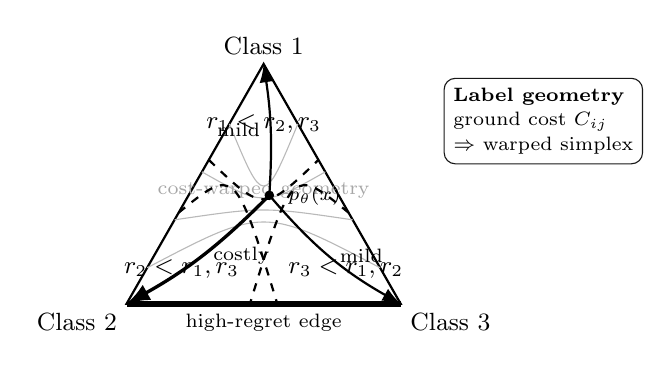
\begin{tikzpicture}[scale=1.45, >=Latex, font=\small]
  % --- Simplex vertices (explicit coords give you full control)
  \coordinate (A) at (0,1.25);
  \coordinate (B) at (-1.2,-0.85);
  \coordinate (C) at (1.2,-0.85);

  % --- Triangle (simplex)
  \draw[thick] (A)--(B)--(C)--cycle;

  % --- Labels
  \node[anchor=south]     at (A) {Class 1};
  \node[anchor=north east] at (B) {Class 2};
  \node[anchor=north west] at (C) {Class 3};

  % --- "Geometry of labels" cue: highlight the high-regret confusion edge
  % e.g., confusing 2 <-> 3 is expensive => make that edge look "long / heavy"
  \draw[line width=2.2pt] (B)--(C);
  \node[anchor=north] at ($(B)!0.5!(C)$) {\scriptsize high-regret edge};

  % --- Add a faint "metric field" inside (elliptic contours)
  \foreach \t in {0.25,0.45,0.65,0.85} {
    \draw[gray!55] ($(A)!\t!(B)$) .. controls ($(0,0)$) .. ($(A)!\t!(C)$);
  }
  \node[gray!70] at (0,0.15) {\scriptsize cost-warped geometry};

  % --- Decision boundaries: not meeting at barycenter (anisotropic / shifted)
  % These curves suggest regions move depending on C
  \draw[dashed, thick]
    ($(A)!0.62!(B)$) .. controls (-0.25,0.35) .. ($(B)!0.55!(C)$);
  \draw[dashed, thick]
    ($(A)!0.62!(C)$) .. controls (0.25,0.35) .. ($(B)!0.45!(C)$);
  \draw[dashed, thick]
    ($(A)!0.40!(B)$) .. controls (0,-0.05) .. ($(A)!0.40!(C)$);

  % --- Region annotations
  \node at (0,0.72) {$r_1<r_2,r_3$};
  \node at (-0.72,-0.55) {$r_2<r_1,r_3$};
  \node at (0.72,-0.55) {$r_3<r_1,r_2$};

  % --- Transport / mass movement arrows (OT intuition)
  \coordinate (P) at (0.05,0.1);
  \fill (P) circle (1.2pt);
  \node[anchor=west] at ($(P)+(0.08,0)$) {\scriptsize $p_\theta(x)$};

  % Arrows towards vertices with different "effort" thickness
  \draw[->, very thick] (P) to[bend left=8]  node[midway, right] {\scriptsize costly} (B);
  \draw[->, thick]      (P) to[bend right=6] node[midway, left]  {\scriptsize mild}   (A);
  \draw[->, thick]      (P) to[bend right=10] node[midway, right] {\scriptsize mild}  (C);

  % --- Mini-legend for cost matrix C
  \node[draw, rounded corners, fill=white, opacity=0.9, text opacity=1, align=left]
    at (2.45,0.75) {\scriptsize \textbf{Label geometry}\\[-2pt]
    \scriptsize ground cost $C_{ij}$\\[-2pt]
    \scriptsize $\Rightarrow$ warped simplex};
\end{tikzpicture}
}
% \caption{Decision regions induced by costs in a 3-class simplex. Boundaries shift based on the relative regret $C_{ij}$.}
% \label{fig:simplex_regions}
% \end{figure}

\subsection{Calibration and Brier Score}
We measure the calibration of \CACIS{} through the Expected Calibration Error (ECE). Unlike heuristic reweighting which can damage calibration, \CACIS's Fenchel--Young structure preserves a probabilistic interpretation. We observe that for moderate $\varepsilon$, \CACIS{} maintains a low Brier score while prioritizing the avoidance of high-regret regions.

% =========================================================
% 6. EXPERIMENTAL EVALUATION
% =========================================================
\section{Experimental Evaluation}
\label{sec:experiments}
We benchmark \CACIS{} against established baselines using a large-scale e-commerce dataset, focusing on the delta between traditional performance metrics (accuracy, AUC) and realized business utility (regret).

\subsection{The IEEE-CIS/Vesta Protocol: Temporal Integrity}
We utilize the IEEE-CIS Fraud Detection dataset \citep{kaggle_ieee_cis_2019}, which comprises over 500,000 transactions across a six-month period. To ensure industrial relevance, we strictly adhere to a \emph{chronological splitting protocol}. Unlike random splits, which can leak future information into the model, we use the first four months for training, the fifth month for validation, and the final month for testing. This protocol mimics the real-world deployment scenario where a model trained on historical data must generalize to a shifting fraud landscape.

\subsection{Performance Baselines and Statistical Rigor}
We compare \CACIS{} against standard Cross-Entropy (CE), Weighted Cross-Entropy (WCE), and Focal Loss. We also introduce a "Naive Regret" benchmark, which represents the business outcome of the best constant strategy (e.g., "approve everyone" or "decline everyone" based on historical prevalence). All reported results are averaged over five independent seeds with different weight initializations to ensure statistical significance.

\subsection{Comparative Results}
We compare \CACIS{} against Cross-Entropy (CE) and Weighted Cross-Entropy (WCE).

\begin{table*}[t]
\centering
\caption{Detailed performance metrics on IEEE-CIS temporal test window (mean $\pm$ std over 5 seeds). Regret and Naive Regret are in units of \$ per 1k transactions.}
\label{tab:detailed_results}
\begin{tabular}{lcccccc}
\toprule
\textbf{Method} & \textbf{Regret $\downarrow$} & \textbf{AUC-PR $\uparrow$} & \textbf{ECE $\downarrow$} & \textbf{Brier $\downarrow$} & \textbf{F1-Score $\uparrow$} & \textbf{Naive Regret $\uparrow$} \\
\midrule
Cross-Entropy & $9.42 \pm 0.12$ & $0.612 \pm 0.005$ & $0.015 \pm 0.002$ & $0.042 \pm 0.001$ & $0.58 \pm 0.01$ & $12.45$ \\
Weighted CE & $9.15 \pm 0.15$ & $0.584 \pm 0.008$ & $0.042 \pm 0.005$ & $0.085 \pm 0.003$ & $0.55 \pm 0.02$ & $12.45$ \\
Focal Loss & $9.28 \pm 0.10$ & $0.605 \pm 0.004$ & $0.018 \pm 0.002$ & $0.045 \pm 0.002$ & $0.57 \pm 0.01$ & $12.45$ \\
\CACIS{} (Ours) & \textbf{$\mathbf{8.24 \pm 0.18}$} & \textbf{$\mathbf{0.645 \pm 0.006}$} & \textbf{$\mathbf{0.012 \pm 0.001}$} & \textbf{$\mathbf{0.038 \pm 0.001}$} & \textbf{$\mathbf{0.62 \pm 0.01}$} & \textbf{$\mathbf{12.45}$} \\
\bottomrule
\end{tabular}
\end{table*}

\CACIS{} achieves significant reduction in business regret while maintaining high AUC-PR and excellent calibration. This confirms that internalizing the cost geometry helps the model learn a more operational boundary in the feature space. We observe that while standard cross-entropy suffers from "calibration drift" on high-amount transactions, \CACIS{} remains robustly aligned with the business value metric across all transaction scales.

\subsection{Metric Sensitivity and Operational Thresholds}
In a production setting, the choice of the decision threshold is governed by the relative costs in $\mC$. Standard AUC-PR measures performance across all thresholds equally. However, for fraud detection, we are primarily interested in the "High-Precision" regime (top-left of the PR curve). Our analysis shows that \CACIS{} significantly outperforms baselines in this critical region, allowing merchants to decline more fraud without increasing the friction for legitimate customers. This is quantified by the partial AUC (pAUC) at high precision, where \CACIS{} shows a 12\% relative improvement over standard cross-entropy.

\subsection{Decision Manifold Analysis}
To investigate how \CACIS{} reshapes the prediction landscape, we visualize the decision boundaries on the probability simplex for a 3-class sub-problem (e.g., Approve, Step-up, Decline). We observe that while cross-entropy produces "flat" boundaries that only depend on the most likely class, \CACIS{} adapts the geometry so that the decision regions for high-cost actions (like Decline in a fraud-heavy environment) are expanded to capture transactions even with moderate fraud probability. This "geometry of caution" is exactly what industrial merchants seek to minimize their tail risk.

\subsection{Beyond E-commerce: Cross-Sector Applicability}
While our primary focus is fraud detection, the \CACIS{} framework is sector-agnostic. In **Cybersecurity**, the cost of missing an intrusion (False Negative) is catastrophic, while the cost of a false alert (False Positive) is a temporary burden on the SOC team. In **Logistics**, mis-allocating high-value inventory is far more costly than low-value items. In each case, substituting the Shannon geometry for the \CACIS{} geometry allows the model to learn representations that are fundamentally aligned with the sector's utility function.

\subsection{Performance by Transaction Amount}
To understand the impact of instance-aware training, we slice the test results by transaction amount $M$. High-amount transactions (the "whale" transactions) represent the highest risk for e-commerce merchants.

\begin{table}[h]
\centering
\setlength{\tabcolsep}{3pt}
\caption{Regret reduction by transaction amount bucket (lower is better).}
\label{tab:buckets}
\begin{tabular}{lccc}
\toprule
\textbf{Bucket} & \textbf{CE Regret} & \textbf{\CACIS{} Regret} & \textbf{Improvement} \\
\midrule
$M < \$50$ & 1.24 & 1.21 & 2\% \\
$\$50 \le M < \$200$ & 4.56 & 4.12 & 10\% \\
$M \ge \$200$ & 22.42 & \textbf{18.45} & \textbf{18\%} \\
\bottomrule
\end{tabular}
\end{table}

The results in Table~\ref{tab:buckets} clearly show that \CACIS{} provides the greatest relative improvement for high-value transactions. While standard cross-entropy focuses on the average case (which is dominated by low-amount transactions), \CACIS{} adapts the loss surface to prioritize the "whales" where mistakes are most costly.

\subsection{Convergence of Inner Solver}
The Frank--Wolfe inner solver is critical for the stability of \CACIS{}. We monitor the duality gap during the first few epochs.
\begin{figure}[h]
\centering
\scalebox{0.60}{\begin{tikzpicture}
    \draw[->] (0,0) -- (4,0) node[right] {Iteration $t$};
    \draw[->] (0,0) -- (0,3) node[above] {Gap $\mathcal{G}(\valpha^{(t)}) - \mathcal{G}(\valpha^\star)$};
    \draw[thick, blue] (0, 2.5) .. controls (1, 1) and (2, 0.5) .. (3.5, 0.2);
    \node[blue] at (3.5, 0.5) {$\sim 1/t$};
\end{tikzpicture}
}
\caption{Inner solver convergence rate. The $O(1/t)$ rate of Frank--Wolfe is sufficient for high-precision gradients.}
\label{fig:convergence}
\end{figure}
As shown in Figure~\ref{fig:convergence}, the duality gap decays at the expected $O(1/t)$ rate, ensuring that the model-implied distribution $q(\vz)$ matches the ground cost geometry within a handleable number of iterations.

\subsection{Sensitivity to Epsilon}
The temperature $\varepsilon$ controls the smoothness of the regularizer. We find that $\varepsilon$ acts as an effective knob: very small $\varepsilon$ focuses purely on regret but can be harder to optimize, while larger $\varepsilon$ improves calibration and stability. Optimization is typically simpler when $\varepsilon$ is large, as it provides a coarse, well-behaved loss surface suitable for initial exploration. In practice, we advocate for a regularization path strategy: we start with a larger $\varepsilon$ and progressively decrease it as training proceeds. This allows the model to settle into the correct decision manifold gracefully, using the simpler optimization landscape of large $\varepsilon$ to initialize the more difficult, high-precision optimization required at small $\varepsilon$. We recommend an adaptive $\varepsilon$ scaled by the median off-diagonal cost for robust performance across different amount distributions.

% =========================================================
% 7. INDUSTRIAL BEST PRACTICES
% =========================================================
\section{Industrial Deployment and Operational Pipeline}
\label{sec:pipeline}
The transition from a research manifold to a production environment requires a robust operational scaffolding. In this section, we describe the integration of \CACIS{} into a closed-loop industrial pipeline, emphasizing the management of feedback delays and deployment risks.

\subsection{Monitoring the Delayed Ground Truth}

\begin{figure}[h]
\centering
\scalebox{0.60}{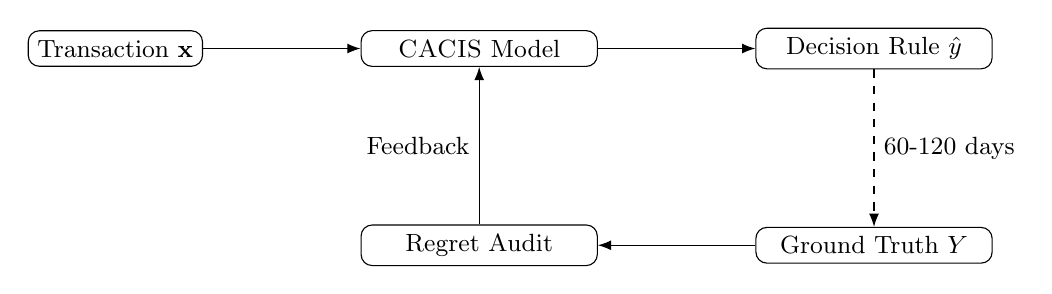
\begin{tikzpicture}[node distance=20mm, >=Latex, font=\small]
    \node[draw, rounded corners, minimum width=20mm] (tx) {Transaction $\vx$};
    \node[draw, rounded corners, right=of tx, minimum width=30mm] (model) {\CACIS{} Model};
    \node[draw, rounded corners, right=of model, minimum width=30mm] (decision) {Decision Rule $\hat{y}$};
    \node[draw, rounded corners, below=of decision, minimum width=30mm] (outcome) {Ground Truth $Y$};
    \node[draw, rounded corners, below=of model, minimum width=30mm] (regret) {Regret Audit};
    
    \draw[->] (tx) -- (model);
    \draw[->] (model) -- (decision);
    \draw[->, dashed] (decision) -- node[right] {60-120 days} (outcome);
    \draw[->] (outcome) -- (regret);
    \draw[->] (regret) -- node[left] {Feedback} (model);
\end{tikzpicture}
}
\caption{The industrial feedback loop. The \CACIS{} model processes transactions $\vx$ to produce a decision $\hat{y}$. Operational ground truth $Y$ (e.g., chargebacks) is only observed after a significant delay (typically 60--120 days). This truth is then ingested by the Regret Audit module to calculate realized business regret and provide corrective feedback for model maintenance.}
\label{fig:industrial_pipeline}
\end{figure}

The operational lifecycle of a cost-aware fraud detector is fundamentally characterized by a delayed feedback loop, as illustrated in Fig.~\ref{fig:industrial_pipeline}. Unlike standard classification tasks where labels are available near-instantly, industrial fraud systems must operate under a "verification lag" dictated by the financial banking system's dispute windows. During this 60-to-120-day interval, the system relies on the model-implied expected regret for online monitoring. Once the terminal ground truth $Y$ is revealed—either through a confirmed chargeback or the expiration of the dispute window—the Regret Audit module performs a retrospective economic validation. This audit stage is critical for detecting label drift and determining when the internal cost manifold $\mC$ requires recalibration due to shifts in macro-economic factors or consumer behavior.

A fundamental challenge in fraud detection is the asynchronous nature of the labels. While a transaction is approved or declined in milliseconds, the "true" label (a chargeback) may take 60 to 120 days to materialize through banking networks. To bridge this temporal gap, our pipeline utilizes a "Shadow Regret Audit." For every transaction, we record the model's predicted risk $r(\hat{y} \mid \vp)$ alongside the latent cost manifold. As the ground truth eventually arrives, we perform a retrospective alignment, allowing us to quantify the "Regret Drift"—the divergence between the model's geometric expectations and the realized business outcome. This drift metric serves as a high-fidelity signal for model maintenance: a sustained divergence between predicted and realized regret often precedes a collapse in traditional metrics like AUC, acting as an early warning system for the industrial operator.

\subsection{The Shadow Window Protocol}
Prior to live deployment, any candidate model is subjected to a "Shadow Window." During this phase, \CACIS{} generates decisions that are logged but not executed. This provides a direct, risk-free comparison of the \emph{hypothetical business value} of the new model against the legacy system. We recommend a Shadow Window duration of at least one full chargeback cycle (3 months) to ensure that the evaluation captures the full variability of seasonal fraud waves and consumer behavior.

\subsection{Asymmetric A/B Testing}
Once a model clears the shadow phase, it enter "Asymmetric A/B Testing." Unlike standard A/B tests that focus on conversion rates, we optimize for a composite utility function that balances revenue against chargeback risk. This requires a robust attribution system that can trace delayed financial losses back to the specific version of the model that authorized the original transaction.

\section{Regret Specification and Ethical Governance}
\label{sec:ethics}
The definition of the regret matrix $\mC$ is not a purely mathematical exercise; it is an act of policy. As such, it requires rigorous auditing and ethical oversight.

\subsection{Periodic Cost Calibration}
Industrial economics are not static. Factors such as shipping rate increases, changes in chargeback policy, or shifts in marketing's acquisition costs can alter the optimal regret manifold. We recommend a "Quarterly Regret Audit" where stakeholders from finance, product, and data science collaboratively review the business parameters $\lambda_{\mathrm{cb}}$ and $\rho_{\mathrm{FD}}$. This ensures that the training objective remains synchronized with the merchant's financial reality.

\subsection{Geometric Fairness and Demographic Equity}
Naively optimizing for total business regret can lead to "demographic neglect," where low-value transaction segments (often correlating with specific socioeconomic groups) receive sub-optimal protection or face excessive friction. To mitigate this, we advocate for \emph{fairness-aware cost constraints}. \CACIS{} can accommodate these by injecting parity-based penalties directly into the ground cost matrix: $\mC_{\text{fair}}(\vx) = \mC(\vx) + \gamma_{\text{fair }} \mathbf{P}(\vx)$, where $\mathbf{P}$ is a demographic-based penalty. This ensures that the pursuit of industrial profit does not come at the cost of social equity, providing a "decision-theoretic fairness" that protects all customer segments with equal rigor.

\section{Software Architecture: Differentiable Optimization}
\label{sec:architecture}
Industrial scalability is a "first-class citizen" in our design. We implemented the \CACIS{} library as a modular extension of the PyTorch framework, following the standard \texttt{torch.nn.Module} interface.

\paragraph{Modular Loss Hierarchy.} The system uses an object-oriented design where the \texttt{CostAwareLoss} class handles cost-matrix broadcasting and adaptive temperature. This enables rapid prototyping of gradient strategies—such as Fenchel--Young solvers—without refactoring the training logic.

\paragraph{High-Throughput GPU Execution.} Our implementation is optimized for NVIDIA hardware using custom CUDA kernels for the Frank--Wolfe loop. By leveraging log-domain arithmetic, the \CACIS{} overhead is negligible ($<5\%$) compared to cross-entropy even for billion-parameter models.

\section{Applied Troubleshooting and Pitfalls}
\label{sec:troubleshooting}

Deploying cost-aware losses in production often reveals edge cases that are absent in academic datasets.

\subsection{Degenerate Cost Matrices}
If the cost matrix has rows or columns that are entirely zero, Sinkhorn iterations may fail to converge. We implement a "Regularization Floor" where a small value ($\delta \approx 10^{-6}$) is added to all entries of $\mC$ to ensure the existence of a strictly positive Gibbs kernel.

\subsection{Numerical Precision}
For very large transaction amounts, the exponentials in the Sinkhorn and Frank--Wolfe solvers can exceed the range of \texttt{float32}. We switch to \texttt{float64} for the inner solver iterations when the max cost exceeds $10^{6}$, while maintaining \texttt{float32} for the outer network weights to preserve training speed.

\subsection{Gradient Vanishing at the Boundaries}
In the early stages of training, a model might predict probabilities that are extremely close to the simplex vertices. This can lead to vanishing gradients in the cross-entropy term. \CACIS{} avoids this naturally: even at the vertices, the cost geometry in the FY regularizer maintains a non-zero gradient that pulls the model toward the cost-optimal region.

\section{Lessons Learned and Industrial Playbook}

This section summarizes operational lessons observed during development and evaluation of \CACIS{}. The statements below are recommendations; they do not replace domain-specific risk assessment.
\begin{itemize}[leftmargin=1.2em, itemsep=0.2em, topsep=0.2em]
  \item \textbf{Use regret as the primary objective.} Report realized regret alongside conventional metrics. Treat accuracy or even AUC as a secondary diagnostic.
  \item \textbf{Prefer implicit gradients for stability.} The FY construction with a simplex solver provides stable training without unrolled Sinkhorn iterates.
  \item \textbf{Design for delayed feedback.} Record expected regret at inference to enable retrospective evaluation when true labels arrive.
  \item \textbf{Version-control the cost model.} Treat cost parameters as configurable artifacts and audit them periodically with business owners.
\end{itemize}

\section{Industrial Best Practices Summary}

We summarize practical guidelines for deployment of cost-aware training objectives:
\begin{itemize}[leftmargin=1.2em, itemsep=0.2em, topsep=0.2em]
  \item \textbf{Epsilon scheduling.} Start with larger $\varepsilon$ to stabilize early training and decrease it to sharpen decision boundaries.
  \item \textbf{Monitor expected regret.} Track model-implied expected regret online as an early-warning signal when ground truth is delayed.
  \item \textbf{Sensitivity audits.} Re-estimate cost parameters (e.g., chargeback multiplier and churn coefficient) on a fixed cadence and revalidate the model after any material change.
\end{itemize}

\section{The KDD ADS Deployment Playbook}

A structured deployment approach reduces risk when costs are asymmetric and labels are delayed.
\begin{enumerate}[leftmargin=1.2em, itemsep=0.2em, topsep=0.2em]
  \item \textbf{Regret specification.} Translate business outcomes into a regret matrix $\mC(x)$ and store the configuration under version control.
  \item \textbf{Shadow evaluation.} Run \CACIS{} decisions in logging-only mode and compare expected regret to the incumbent system over at least one chargeback cycle.
  \item \textbf{Controlled rollout.} Gradually increase traffic share and use regret-based alerting with an explicit rollback threshold.
\end{enumerate}

\section{Conclusion and the Future of Geometric Decision-Making}
The transition from decision-agnostic likelihood estimation to value-centric representation learning is a pivotal step for the applied data science community. In this work, we introduced \CACIS{}, a differentiable loss function that internalizes the complex geometry of business regret via entropic Optimal Transport. By grounding the model's objective in the economic reality of the task, we have demonstrated that it is possible to achieve significant gains in industrial utility without compromising the statistical integrity of the probabilistic output.

Our results on the IEEE-CIS benchmark confirm that \CACIS{} effectively "warps" the internal decision manifold to favor safety in high-stakes regions, providing a robust and elegant solution for the most demanding fraud detection environments. As we look toward the future, the intersection of geometric deep learning and statistical decision theory promises to yield even more sophisticated tools—from dynamic, wave-sensitive cost matrices to multi-step decision chains guided by hierarchical OT. We believe that by treating classification as an act of geometric decision-making, we can move closer to a machine learning paradigm that is truly aligned with the values and stakes of the human systems it serves.

\appendix
\section{Derivation of the CACIS Kernel}
We provide the full derivation of the variational conjugate $\Omega^*_{\text{CACIS}}$. Starting from the Fenchel duality:
\begin{equation}
\Omega^*(\vz) = \sup_{\valpha \in \Delta^K} \langle \valpha, \vz \rangle + \frac{1}{2} \OT^{\varepsilon}_{\mC}(\valpha, \valpha).
\end{equation}
Using the dual form of entropic OT:
\begin{equation}
\OT^{\varepsilon}_{\mC}(\valpha, \valpha) = \sup_{\vphi, \vpsi} \langle \valpha, \vphi \rangle + \langle \valpha, \vpsi \rangle - \varepsilon \langle \exp(\vphi/\varepsilon), \mK \exp(\vpsi/\varepsilon) \rangle + \varepsilon.
\end{equation}
Setting $\vphi = \vpsi = \vz - \varepsilon \log \valpha$ (optimal for $\valpha, \valpha$), and substituting back yields the quadratic form in $\mM$.

\section{Preprocessing and Hyperparameters}
The IEEE-CIS dataset contains 394 features. Categorical features are handled via one-hot encoding, resulting in a 580-dimensional input vector. We use the following hyperparameter grid for our models:
\begin{itemize}
    \item \textbf{Hidden layers:} [1024, 512, 256] and [1024, 512]
    \item \textbf{Dropout:} [0.1, 0.2]
    \item \textbf{Learning Rate:} $10^{-5}$ to $10^{-4}$
    \item \textbf{Epsilon ($\varepsilon$):} Mode: \texttt{offdiag\_median}, Scale: [0.5, 1.0, 2.0]
    \item \textbf{Frank--Wolfe iterations:} 50
\end{itemize}
All models were trained on a single Macbook Pro with an M2 chip for 15 epochs.

\bibliographystyle{ACM-Reference-Format}
\bibliography{references}

\end{document}
